\section{Augmented Reality in Educational Environments}

\subsection{Definition of "Augmented Reality"}
Although the term 'Augmented Reality' was coined in 1990 by Tom Caudell, a former Boeing researcher, the concept of augmenting the real world with virtual data was initially used by a number of applications in the late 1960s and 1970s. Since the 1990s, AR was used by some large companies in purpose of visualization and training. Nowadays, the rising power of personal computers and mobile devices enable the concept of AR to be delivered to traditional educational environments such as schools and universities. \autocite [cf.][21]{Johnson.2010} 
\begin{figure}[ptbh]
    \centering
    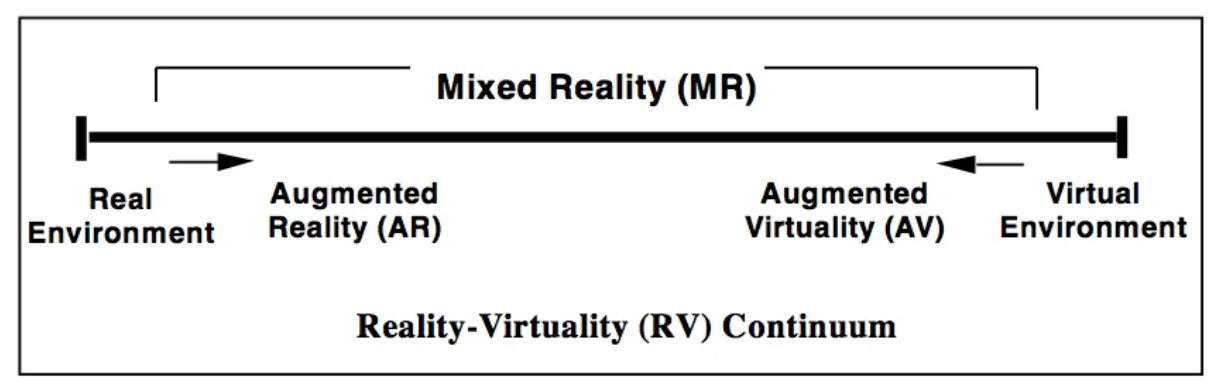
\includegraphics[width=\linewidth]{figures/rvc.png}
    \caption[Reality-Virtuality Continuum]{Reality-Virtuality Continuum}
    \label{fig:RealityVirtualityContinuum}
\end{figure}

During the last years the term 'Augmented Reality' has been given different meanings by varying researchers. \autocite [cf.][42]{Wu.2013} \cite{Milgram.1994b} defined AR on the basis of the reality-virtuality continuum (\ref{fig:RealityVirtualityContinuum}) as "augmenting natural feedback to the operator with simulated cues". \autocite[283]{Milgram.1994b} The reality-virtuality continuum (\ref{fig:RealityVirtualityContinuum}) allows us to distinguish the concept of AR to related concepts such as Virtual Reality (VR) where "the participant observer is totally immersed in a completely synthetic world" \autocite[283]{Milgram.1994b} or Augmented Virtuality (AV) where "the the primary world being experienced is in fact [...] predominantly 'virtual'"\autocite[4]{Milgram.1994} and augmented with information from the real world. In addition, \cite{Milgram.1994b} mention a more restricted definiton where AR is seen as "form of virtual reality where the participant's head-mounted display is transparent, allowing a clear view of the real world". \autocite[283]{Milgram.1994b} As suggested by educational researchers,\autocite[cf.][42]{Wu.2013} we reject the idea that the concept of AR is limited to any type of technology. Therefore, we broadly define AR referring to \cite{Klopfer.2008} as "a situation in which a real world context is dynamically overlaid with coherent location or context sensitive virtual information"\autocite[205]{Klopfer.2008} and regard it as a concept which is based on and realized by but conzeptualized beyond technology.

\subsection{Five Directions of Augmented Reality in Educational Environments}
There are several different ways how the concept of AR can be implemented in educational environments. \autocite {Yuen.2011}\mulcit\autocite {Lee.2012} The Five Directions by \cite{Yuen.2011} enable us to classify the AR applications we are investigating in our systematic literature review into five groups which are introduced in the following. This classification helps us to find out how the benefits of AR in educational environments differ dependent on the regarded type of AR application.
\heading{Discovery-based Learning}
AR is often used in applications that enable discovery-based learning. Therefore, the user is provided with information about a real-world place while simultaneously regarding the object of interest. This type of application is often used in museums, in astronomical education or at historical places.
\heading{Objects Modeling}
AR is also used in objects modeling applications. These applications allow students to receive immediate visual feedback of how a given item would look like in a different setting. Some applications also allow students to design virtual objects in order to investigate their physical properties or interactions between objects. This type of application is also used in architectural education.
\heading{AR Books}
AR books are books which offer students 3D presentations and interactive learning experiences through AR technology. The books are augmented with the help of technological devices such as special glasses. The first implementations of AR books show that this kind of medium is likely to appeal to digital native learners which makes it an appropriate educational medium even at the primary level.
\heading{Skills Training}
The support of training individuals in specific tasks is described by the term 'Skills Training'. Especially mechanical skills are likely to be supported by AR skills training applications. AR skills training applications are used for example in airplane maintenance, where each step of a repair is displayed, necessary tools are identified and textual instructions are included. Skills training applications are often realised with head-mounted displays. 
\heading{AR Gaming}
Video Games offer powerful new opportunities for educators which have been ignored for many years. \autocite{Squire.2003} Nowadays, educators have recognized and often use the power of games and gamification in educational environments. AR technology enables the development of games which take place in the real world and are augmented with virtual information. AR games can give educators powerful new ways to show relationships and connections. In addition, they provide educators with highly interactive and visual forms of learning.